\documentclass[11pt, a4paper]{article}
\usepackage[a4paper, margin=1in]{geometry}


\usepackage{adjustbox}
\usepackage{mathtools}
\usepackage{amsmath}
\usepackage{amssymb}
\usepackage{amsthm}

\usepackage{pgfplots}
\usepackage{listings}
\usepackage{color}
\usepackage{tikz}
\usepackage{multirow}

\usepackage{textcomp}
\usepackage{soul}

\usepackage[hidelinks]{hyperref}
\pgfplotsset{width=7.5cm,compat=1.12}
\usepgfplotslibrary{fillbetween}
\usepackage[makeroom]{cancel}
\title{\bf{Homework \textnumero 8}}
\author{Author: David Oniani
\\
\ \ \ Instructor: Dr. Eric Westlund}
\date{March 6, 2019}

\usepackage{listings}
\usepackage{color}

%%%%%%%%%%%%%%% S E T S %%%%%%%%%%%%%%%
\newcommand{\nats}{\mathbb{N}}
\newcommand{\ints}{\mathbb{Z}}
\newcommand{\rats}{\mathbb{Q}}
\newcommand{\reals}{\mathbb{R}}
\newcommand{\irrats}{\mathbb{I}}

\newcommand{\pnats}{\mathbb{N}^+}
\newcommand{\pints}{\mathbb{Z}^+}
\newcommand{\prats}{\mathbb{Q}^+}
\newcommand{\preals}{\mathbb{R}^+}
\newcommand{\nreals}{\mathbb{R}^-}

\newcommand{\nints}{\mathbb{Z}^-}
\newcommand{\nrats}{\mathbb{Q}^-}
%%%%%%%%%%%%%%%%%%%%%%%%%%%%%%%%%%%%%%%

% Calligraphy
\newcommand\und[1]{\underline{\smash{#1}}}

% Operators
\DeclarePairedDelimiter\abs{\lvert}{\rvert}
\DeclarePairedDelimiter\ceil{\lceil}{\rceil}
\DeclarePairedDelimiter\floor{\lfloor}{\rfloor}

% Other
\newcommand{\rarr}{\rightarrow}

\definecolor{dkgreen}{rgb}{0,0.6,0}
\definecolor{gray}{rgb}{0.5,0.5,0.5}
\definecolor{mauve}{rgb}{0.58,0,0.82}
\definecolor{backcolour}{rgb}{0.95,0.95,0.92}

\lstset{
backgroundcolor=\color{backcolour},
aboveskip=3mm,
belowskip=3mm,
showstringspaces=false,
columns=flexible,
basicstyle={\small\ttfamily},
numbers=left,
numberstyle=\normalsize\color{gray},
keywordstyle=\color{blue},
commentstyle=\color{dkgreen},
stringstyle=\color{mauve},
breaklines=true,
breakatwhitespace=true,
tabsize=4
}


\begin{document}
\maketitle

\begin{itemize}
\item[9.6]
\begin{itemize}
\item[(a)]
Subjects, in this case, would be mangoes in the sample.\\\\
The response variable would be the time to ripening.\\\\
Treatments would be: 80 days and 20 degrees centigrade, 80 days and 30 degrees centigrade, 80 days and 40 degrees centigrade, 95 days and 20 degrees centigrade, 95 days and 30 degrees centigrade, 95 days and 40 degrees centigrade, 110 days and 20 degrees centigrade, 110 days and 30 degrees centigrade, 110 days and 40 degrees centigrade.
In other words, all the combinations of days and degrees of centigrade.\\\\
Below is the table.
\begin{table}[h]
    \centering
    \begin{adjustbox}{max width=\textwidth}
    \resizebox{0.6\linewidth}{!}
    {
        \begin{tabular}{*{7}{|c}|}%%{|c|c|c|c|c|c|c|c|c|c|c|c|c|c|}
        \hline
        & 80 Days  & 95 Days & 110 Days \\ \hline
        20 Degrees & 1 & 2  & 3         \\ \hline
        30 Degrees & 4 & 5  & 6         \\ \hline
        40 Degrees & 7 & 8  & 9         \\ \hline
    \end{tabular}
    }
    \end{adjustbox}
\end{table}

\item[]

\item[(b)]
No, it would not be a good way to assign the mangoes to the treatments.
The reason is that mangoes from the same tree would most likely be similar,
sharing same characteristics and therefore, would show approximately same
time for ripening. Other trees would most likely show different times for rippening
making it very difficult to compare the results and draw the conclusion.
\end{itemize}

\item[]
\item[]

\item[9.7]
It might be health condition, education level etc.
\\
To see the results, however, it would be the best if the state
offered \$500 to only some people (treatment group) and not
give to others (control group). This would make it easy to
see the result/impact of offering \$500 (whether it had a positive
or negative impact).

\item[]
\item[]

\item[9.12]
This design is inferior as at first, the control group will get rid of lurking variables and secondly,
the company will be able to save costs if it finds out that the control group lowers its electricity use
as much as either the meters or charts groups.

\newpage

\item[9.13]
\begin{itemize}
\item[(a)]
It is rather observation study as the researchers had no influece/did not control the diet of the participants.
They just gathered the infromation from a simple observation.

\item[]

\item[(b)]
Observational studies do not show the causal relationship.\\
To show the causal relationship, one must do the experimental study.
\end{itemize}

\item[]
\item[]

\item[9.14]
A double-blind experiment is the one in where neither the subjects nor the researchers who measure know which treatment each subject received.\\\\
A randomized experiment randomly assigns all individuals to a group.\\\\
Placebo-controlled indicates that there is a placebo group. A placebo is a substance or treatment with no active therapeutic effect.
It is also known as a fake drug (it is used to make subjects of the experiment believe that they actually receive drugs).

\item[]
\item[]

\item[9.45]
We can make each player run 100 yards twice. Once without oxygen and once with oxygen.
For each player, we can randomly (flip a coin) choose whether to use oxygen on the first
run or the second run. We should also make sure that players are recovered fully
before the second trial and therefore, we should make sure that there is a gap (say a day or two)
between the trials

\item[]
\item[]

\item[9.46]
\begin{itemize}
\item[(a)]
It is the block experiment.

\item[]

\item[(b)]
Below is the diagram.
\begin{figure}[h]
    \centering
    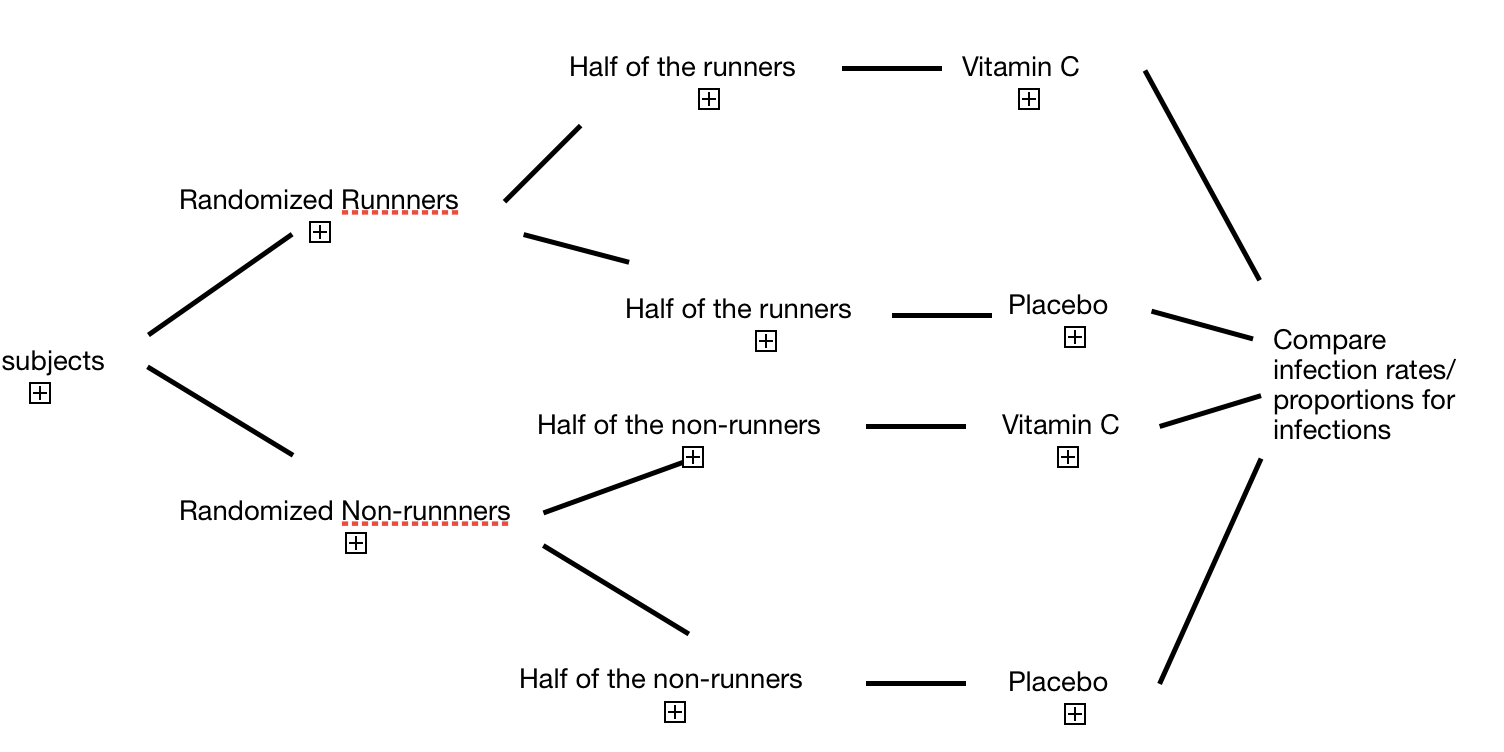
\includegraphics[width=15cm, height=7cm]{diagram_0}
\end{figure}
\end{itemize}

\newpage

\item[9.50]
\begin{itemize}
\item[(a)]
Explanatory variables are beta-carotene, vitamin C, and vitamin E (whether one received either of these vitamins or not).\\
Explanatory variable is cancer (whether one has it or not).

\item[]

\item[(b)]
Below is the diagram.
\begin{figure}[h]
    \centering
    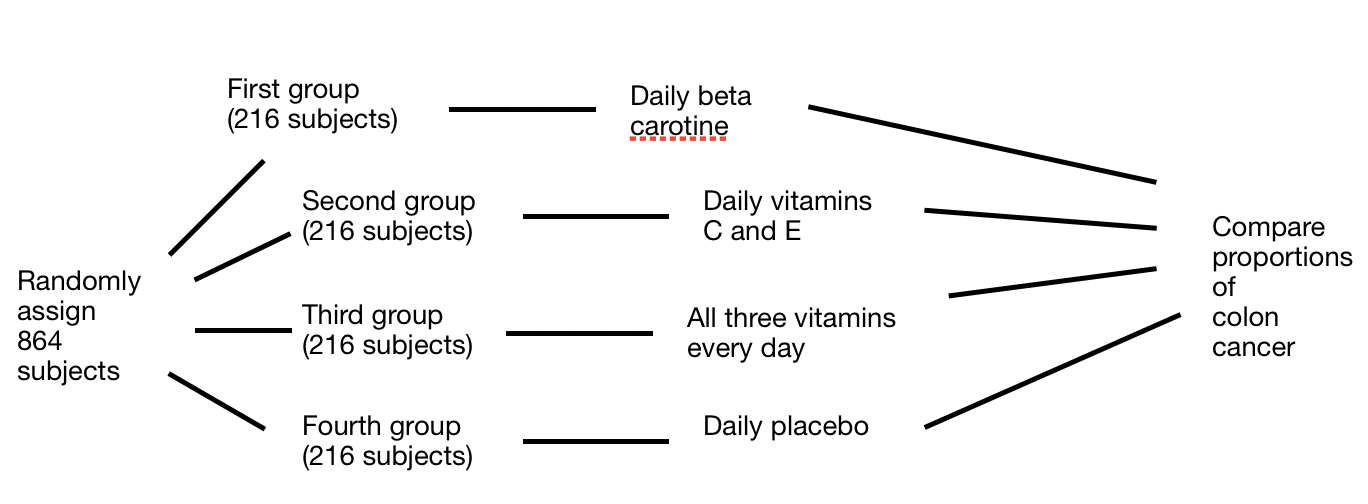
\includegraphics[width=15cm, height=7cm]{diagram_1}
\end{figure}

\item[]

\item[(c)]
It means that neither these 864 subjects nor the researchers
knew which treatment each subject received.

\item[]

\item[(d)]
It means that the differences was so small that they are most probably caused by chance.

\item[]

\item[(e)]
Income, Health, Eating habits, whether one is a smoker or not, etc.
\end{itemize}

\end{itemize}

\end{document}
